\section*{Практические вопросы}

Решение оформлено на отдельном листе бумаге, прилагающемуся к отчету.

\section*{Теоретические вопросы}
\setcounter{page}{2}
% Все данные в lisp представляются в форме символьных выражений S-выражений.

% cons == construct (строить) (Городняя: consolidation (укрепление))
% СAR == Contents of Address Register
% CDR == Contents of Decrement Register 

% eval - выполняет двойное вычисление своего аргумента.

% Единая форма записи программы и данных.

% Лисп-программа представляет собой последовательность атомов или списков, 
% которые можно вычислить и получить значение.

% Вместо общепринятой в математике записи обращений к функциям
% вида f(x,y) в Лиспе используется нотация, при которой имя функции
% стоит не перед аргументными скобками, а внутри них, вместе с
% аргументами, которые разделяются уже не запятыми, а пробелами:
% (f x y). Именно за счёт этого достигается синтаксическое единообразие
% программы и данных.

% \begin{lstlisting}
% x => (GAMMA (15))

% (eval (cons (quote car) (quote (x)))) => GAMMA
% 		|---------(car x)---------|

% \end{lstlisting}

\subsection*{1. Элементы языка.}

Элементами языка являются атомы и точечные пары.

\textbf{Атомы} представляю из себя:
\begin{enumerate}
	\item Символы - синтаксически представляется как набор букв и цифр, начинающийся с буквы.
	\item Специальные символы - \{T, Nil\}.
	\item Самоопределимые атомы - натуральные, дробные и вещественные числа, а также строки, заключенные в двойные апострофы. 
	% Их значение переопределить нельзя.
\end{enumerate}

Атомы обычно выглядит как последовательность букв или цифр.

Примеры атомов:
\begin{lstlisting}
	B
	CAT
	123
	2/3
	"abc"
\end{lstlisting}

\textbf{Специальные символы:}

\begin{enumerate}
	\item \textbf{T} - Константа. обозначает логическое значение <<истина>>. Истинным значением является все, что отличное от Nil.
	\item \textbf{Nil} - <<ложь>>. Также обозначает пустой список. Записи nil и () эквивалентны. Являются синтаксисом пустого списка.
\end{enumerate}

Более сложные данные - списки и точечные пары. строятся из унифицированных структур -- блоков памяти -- бинарных узлов.


\textbf{Точечная пара} -- (A . B). Строится с помощью бинарных узлов.   

\begin{lstlisting}
	Точечная пара ::= (<атом>.<атом>) |
		     (<атом>.<точечная пара>) |
	  		 (<точечная пара>.<атом>) |
	   		 (<точечная пара>.<точечная пара>)	
\end{lstlisting}

Пример точечной пары:
\begin{lstlisting}
	(A . (B . (C . (D . Nil))))
\end{lstlisting}
Облегченная форма записи:
\begin{lstlisting}
	(A B C D)
\end{lstlisting}

\begin{figure}[ht!]
	\centering{
		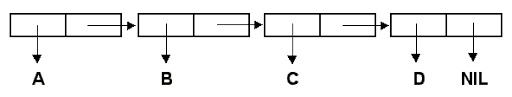
\includegraphics[width=0.9\textwidth]{img/img1}
		\caption{Представление в памяти (A B C D).} }
\end{figure}

\textbf{Представление в памяти:}

\begin{enumerate}
	\item \textbf{(A . B)}
	\begin{figure}[ht!]
		\centering{
			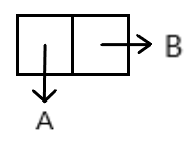
\includegraphics[width=0.2\textwidth]{img/img3}
			\caption{Представление в памяти (A . B).} }
	\end{figure}
	\item \textbf{(A B)} - экономия памяти, но проблема при рекурсивной обработке (т.к. не сможем идентифицировать конец, как Nil)
	\begin{figure}[ht!]
		\centering{
			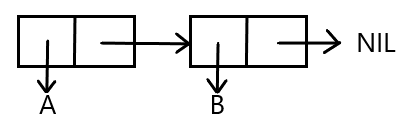
\includegraphics[width=0.5\textwidth]{img/img2}
			\caption{Представление в памяти (A B).} }
	\end{figure}
\end{enumerate}

Вся информация (данные и программы) в Lisp представляется в виде символьных выражений -- S-выражений.
\begin{lstlisting}
	S-выражение ::= <атом> | <точечная пара>
\end{lstlisting}

Список является частым случаем S-выражения.

%S-выражение представлено 

%\begin{figure}[ht!]
%	\centering{
%		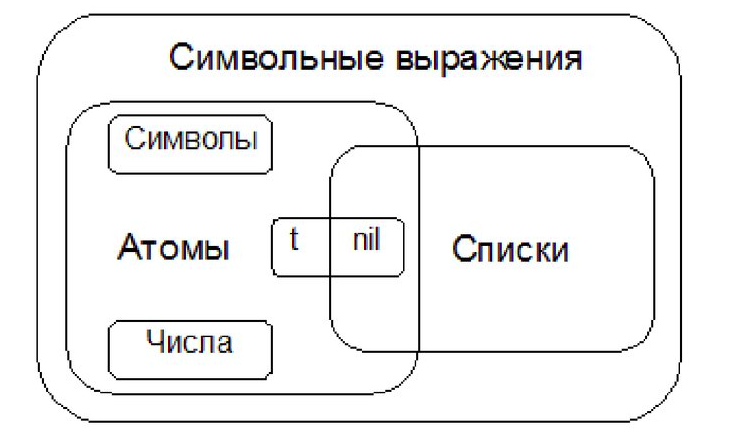
\includegraphics[width=0.5\textwidth]{img/img4}
%		\caption{S-выражение} }
%\end{figure}

\textbf{Список} - динамическая структура данных, которая может быть пустой или непустой. Если она не пустая, то состоит из двух элементов:

1. Головы -- S-выражение.

2. Хвоста -- список.

Список представляет из себя заключенную в скобки
последовательность из атомов, разделенных пробелами, или списков.
Любой список является программой - его нужно вычислять.

%Примеры списков:
%\begin{lstlisting}
%	(A B C)
%	(1 2 3)
%	((A B) (C D))
%\end{lstlisting}

%Структура — это объединение нескольких объектов, возможно, различного типа под одним именем, которое является типом структуры. 

Структуры -- тотечная пара и список


\subsection*{2. Синтаксис.}

Lisp является регистронезависимым языком. Lisp использует префиксную нотацию.

Универсальным разделителем, между атомами, является пробел. В начальных версиях была предложена запятая, но она не прижилась.

Наличие скобок является признаком структуры -- списка или точечной пары.
% Ограничитель - круглые скобки.


Любая структура заключается в круглые скобки, в памяти представляется как списковая ячейка, хранящая два указатели: на голову (первый элемент) и на хвост (все остальное).

(A . B) -- точечная пара.

(A) -- список из одного элемента.

() или Nil -- пустой список.

Одноуровневый список:
\begin{lstlisting}
	(A B C D)
\end{lstlisting}

Структурированный список:
\begin{lstlisting}
	(A (B C) (D E))
\end{lstlisting}

\subsection*{3. Особенности языка Lisp. Символ апостроф}
Особенности языка Lisp: только символьная обработка данных.

От других языков программирования Lisp отличается следующими свойствами:

\begin{enumerate}
\item Используется символьная обработка данных.

\item Нет типизации (без типовый язык).

\item Программы, написанные на Lisp, представляются в виде списков.

\item Программа может быть представлена в виде данных, поэтому программа может модифицировать сама себя.

\item Память выделяется блоками. Lisp сам распределяет память.
\end{enumerate}




Символ апостроф -- синоним quote.

\textbf{quote} -- блокирует вычисление своего аргумента. В качестве своего значения выдаёт сам аргумент, не вычисляя его. Перед константами -- числами и атомами T, Nil можно не ставить апостроф.
% т.к. значением любой константы является она сама.

Пример использования quote:
\begin{lstlisting}
	(quote (car (A B C))) => (car (A B C))
\end{lstlisting}



Вычисление начинается с внешней функции quote, которая возвращает аргумент в неизмененном виде.

\subsection*{4. Базис Lisp}

Базис Lisp 
\begin{itemize}
	\item атомы и структуры (представляющиеся бинарными узлами);
	\item базовые (несколько) функций и функционалов: встроенные — примитивные
	функции (atom, eq, cons, car, cdr); специальные функции и функционалы (quote,
	cond, lambda, eval, apply, funcall).
\end{itemize}

\begin{itemize}
	\item atom проверяет, является ли объект, переданный в качестве аргумента, атомом.
	
		\begin{lstlisting}[language=Lisp]
		(atom 'a) ;; t
		(atom '(a b c)) ;; nil
		\end{lstlisting}
	
	\item eq проверяет идентичность двух символов
	
		\begin{lstlisting}[language=Lisp]
		(eq 'a 'b) ;; nil
		(eq 'a 'a) ;; t
		\end{lstlisting}
	
	\item cond (от англ. condition -- условие). Нет фиксированного количества аргументов. 
	
		Каждый аргумент это список, голова которого рассматривается как условие, в случае если оно истинно, то хвост рассматривается как результат.
		
		\begin{lstlisting}[language=Lisp]
		(cond ((eq 'A 'B) 'yes)
			(T 'not)) ;; NOT
		\end{lstlisting}
	
	\item eval выполняет двойное вычисление своего аргумента.
	
		\begin{lstlisting}[language=Lisp]
		(eval (cons (quote car) (quote ('(A B))))) 
		\end{lstlisting}
	
	
	\item apply функция, аргументом которой является функция. Данная функция требует функцию и список ее аргументов и возвращает результат этой функции с заданными аргументами. 
	
		\begin{lstlisting}[language=Lisp]
		(apply #'+ '(1 2 3))
		(apply #'+ 1 2 '(1 2 3))
		\end{lstlisting}
	
	
	\item funcall аналогично apply, но не требует, чтобы аргументы были упакованы в список.
	
	
		\begin{lstlisting}
		(funcall #'+ 1 2 3)
		(funcall #'+ 1 2 1 2 3)
		\end{lstlisting}

\end{itemize}

Ядро -- основные действия, которые наиболее часто используются. <<Ядро>> шире, чем <<базис>>.

%%%%%%%%%%%%%%%%%%%%%%%%%%%%%%%%%%%%%%%%%%%%%%


%\subsection*{5. Что такое рекурсия и примеры из lisp}

%\textbf{Рекурсия} - это ссылка на описываемый объект в процессе его описания.

% Городняя:
%Примером рекурсии в lisp служит S-выражение, которое может быть атомом, либо заключенная в скобки пара состоящая из S-выражений (разделенных точкой).

%Примером может служить еще список, так как непустой список состоит из головы и хвоста, а хвост в свою очередь может быть списком.

\subsection*{5. Функция}

Функцией называется правило, по которому каждому значению одного или нескольких аргументов ставится в соответствие конкретное значение результата.

Функция в Lispе есть однозначное отображение множества исходных данных на множество её значений. У функции может быть произвольно много аргументов, от нуля до любого конечного числа, но обязательно должно быть хотя бы одно значение

Функционалом, или функцией высшего порядка называется функция, аргументом или результатом которой является другая функция.


\subsection*{7. Классификация функций}

%\begin{enumerate}
	%\item Чистые математические функции - имеет фиксированное количество аргументов и один результат.
	%\item Специальны функции - произвольное количество аргументов.
	%\item Псевдофункции - создают эффект на экране.
	%\item Рекурсивные функции.
	%\item Функции с вариантными значениями, которые возвращают одно значение.
	%\item Функции высших порядков - используются для построения синтаксически управляемых программ. %%(абстракции языка)
%\end{enumerate}

Классификация базисных функций:
\begin{itemize}
	\item селекторы (car cdr)
	\item конструкторы (cons list)
	\item предикаты (atom, consp, listp, null, numberp, oddp)
\end{itemize}


\subsection*{8. CAR и CDR}

Список в языке Lisp представлен одним бинарным узлом, который хранит два указателя (на голову и хвост). 

CAR и CDR являются базовыми функциями доступа к данным. 

CAR принимает точечную пару или пустой список в качестве аргумента и возвращает первый элемент или nil, соответственно. 

CDR принимает точечную пару или пустой список и возвращает список состоящий из всех элементов, кроме первого. Если в списке меньше двух элементов, то возвращается Nil.


\subsection*{9. LIST и CONS}
LIST и CONS являются функциями создания списков (cons – базовая, list – нет).
Функция cons (принимает только два аргумента) создает списочную ячейку и устанавливает два указателя на аргументы. 

Функция list принимает переменное число аргументов и возвращает список, элементы которого – переданные в функцию аргументы.

% car указатели этих ячеек устанавливаются на агрументы, с помощью cons указателей связывают списковые ячейки, последний указатель выставляется в Nil.


Например список '(open close halph) из задания 1 можно представить как:
(cons 'open (cons 'close (cons 'halph nil))) 
или (list 'open 'close 'halph).



%Идентификатор - это подкласс атомов, используемых при именовании неоднократно используемых объектов программы - функций и переменных. Предполагается, что идентифицируемые объекты размещаются в памяти так, что по идентификатору их можно найти.

%Переменная - это подкласс идентификаторов, которым сопоставлено многократно используемое значение, ранее вычисленное в подходящем контексте. Подразумевается, что одна и та же переменная в разных контекстах может иметь разные значения. Таким образом, класс форм - это объединение класса переменных и подкласса списков, начинающихся с QUOTE, COND или с представления некоторой функции.
%<аргумент> ::= <форма>
%Форма - это выражение, которое может быть вычислено.


%Куча как структура данных – не просто куча. Термин возник из противопоставления стека как структуры данных, которая реализует определенный алгоритм обслуживания, и кучи, которая представляет просто набор чего-то (в нашем случае-областей памяти).